% Nama Kelompok : 
% Kelas : D4 TI 1A
% Anggota : 
% 1. Harun   	1174027
% 2. Fahmi   	1174021
% 3. Kukuh		1174016
% 4. Izzah		1174013
% 5. Rizal		1174014
% 6. Lawinner	1174030





Artikel tentang Bilangan Oktal
\Section{Penjelasan Singkat}
Oktal adalah sebuah sistem bilangan berbasis delapan. Sistem bilangan ini terdiri dari 0,1,2,3,4,5,6,7 dan bilangan ini biasanya dikonversi dari biner yang berkelompok setiap 3 bit. Sistem ini mempersingkat tulisannya, agar menjadi tidak terlalu panjang. Cara baca sistem ini dari ujung paling kanan (LSB kepanjangan dari Least Significant Bit).

	\ref{Posisibilanganoktal}
	\begin{figures}[ht]
	\centerline{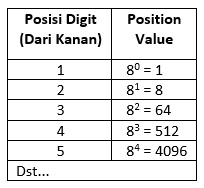
\includegraphics[width=1\textwidth]{figures/Posisibilanganoktal.JPG}}
	\caption{Perhitungan dari kanan}
	\label{Posisibilanganoktal}
	\end{figures}

Contoh contoh bilangan Oktal,
Misalnya : 
Biner Oktal
000 000 00
000 001 01
000 010 02
000 011 03
Misalnya bilangan oktal 3 adalah hasil dari pengelompokkan dari 000 011, perhitungan secara manual dapat dibuktikan dengan cara seperti berikut ini :
(1 x 21 )+(1 x 20 ) = (1×2)+(1×1) = 3

\section{Cara menghitung}
Dengan menggunakan software ms excel kita dapat melakukan konversi bilangan oktal ke bilangan heksadesimal, bilangan desimal atau pun bilangan biner.
 	\subsection{penjumlahan pada Oktal}
 ada beberapa ketentuan yang perlu kalian ketehui dalam penjumlahan bilangan oktal.dimana semua ketentuan akan digunakan pada pengurangan dan perkalian.kalau kalian belum paham betul tentang penjumlahan,saya sarankan jangan mempelajari pada tahap pengurangan dan perkalian.karena walaupun terlihat susah,namun sebenarnya sangat mudah.kunci utamanya yang perlu kalian pahami dan mempelajari ini adalah teliti,semangat da pantang menyerah.
 Hal hal yang harus paling penting harus diketahui antara lain sebagai berikut  :
1. Setiap masing - masing basis harus ditambahkan secara desimal.
2. Setelah itu , kalian harus  mengubah dari hasil desimal ke oktal.
3. Setelah diubah  , kalian harus menulis hasil dari penjumlahan digit paling kanan ke hasil bilangan oktal.
4. lalu hasil penjumlahan yang dilakukan pada tiap basis terdiri dari 2 digit , bilangan binernya nol dan 1 maka digit paling kiri merupakan  penjumlahan kolom selanjutnya.
Kemudian apabila aku menjelaskannya secara rinci , berdasarkan empat ketentuan itu , kira - kira akan seperti ini 
Soal: tambahkan bilangan 9, 6 dan 2.
Ketentuan pertama:
Tambahkan masing-masing basis secara desimal
9 + 6 + 2 = 17
Ketentuan kedua:
Ubah dari hasil desimal ke oktal.
9(8) + 7(8) + 2(8) = 17(8)
Konversikan kebilangan oktal:
17 mod 8 = 2 sisa 1
=21
Demikian cara penjumlahan berdasarkan keempat ketentuan tersebut.
Dalam hal ini bilangan oktal memiliki patokan, Yaitu sebagai berikut.

	\ref{tabelpertambahanbilanganoktal}
	\begin{figures}[ht]
	\centerline{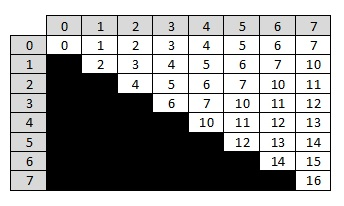
\includegraphics[width=1\textwidth]{figures/tabelpertambahanbilanganoktal.JPG}}
	\caption{Patokan Bilangan}
	\label{tabelpertambahanbilanganoktal}
	\end{figures}

Mungkin ada kalian yang bertanya: Kenapa dari 7 langsung menuju ke angka 10?
Bilangan oktal adalah bilangan yang terdiri dari 0, 1, 2, 3, 4, 5, 6, 7 dimana nilai maksimal adalah 7. Jika lebih dari 7 maka itu  adalah pembawa dan sisanya akan kita jumlahkan pada kolom selanjutnya
1 + 6 = 7. —– > tidak lebih dari 7. Maka tetap.
1 + 7 = 8. —– > carry of 1 dan sisa 0, maka hasilnya adalah 10 (8 mod 8= hasil 1 sisa 0)
2 + 7 = 11. — > carry of 1 dan sisa 1, maka hasilnya adalah 11 (9 mod 8= hasil 1 sisa 1)
Dan seterusnya…

Ada tips yang penting Anda ketahui dan sesuatu yang harus dilaksanakan , saya menyarankan agar kalian berlatih sendiri dengan cara membuat soal dan menjawabnya sendiri . Apabila Anda sering berlatih , maka besar harapan peluang Anda akan sangat mudah untuk memahami dan akan mudah untuk menemukan jawaban-jawaban dari soal yang sangat rumit sekalipun .

Pengurangan Pada Bilangan Oktal
Sekarang kita dapat mempelajari pengurangan di bilangan oktal. Saya tidak perlu memaparkan dengan jelas karena kalian pasti sudah paham dengan pemaparan sebelum nya dimana kalian berpatok pada tabel.
Contoh:
154 – 127 = 25
Coba kalian hitung dengan kalkulator bakul beras! Apa perhitungan saya terlihat berbeda?
Lalu bagaimana dengan perhitungan oktal yang seperti ini:
154
127
____-
 
140 + (8 + 4)                        140 + 12
120 +    7                           120 +   7
__________-                    _______-
                                                20+5
                                                =25

Itulah salah satu contoh dari perhitungan pengurangan bilangan oktal. Dimana kita tidak akan sepenuhnya bergantung dengan kalkulator bakul beras. Walaupun pada Windows disediakan fitur calculator untuk programmer, tapi ada baiknya kalian menghitung dengan usaha kalian sendiri. Kenapa? Supaya kalian lebih teliti dalam memecahkan suatu masalah yang rumit.
 
 